
\begin{center}
	\Huge
	Kryptologi
\end{center}

\section{Kort om kryptologi}


Vi vil begynde med at skabe os en forståelse for, hvad kryptologi det er. Dette vil vi gøre gennem tænkte eksempler, hvor vi løbende introducerer terminologi. Vi vil starte med at introducere et simpelt \textit{kryptosystem}, der beskriver idéen bag kryptologi, men har store sikkerhedsbrister. Dette er det såkaldte \textit{Cæsar-chiffer}, som efter sigende skulle være udtænkt af Julius Cæsar. Et eksempel på et mere berømt kryptosystem er Enigma, der under anden verdenskrig blev brugt af Nazityskland til at sende hemmelige beskeder indbyrdes. 

\subsubsection*{Terminologi}
Begrebet kryptologi dækker overordnet over to begreber: Det at skabe kryptosystemer, som Cæsar-chifferet eller Enigma, som vi kalder for \textit{Kryptografi}, og det at bryde eller knække kryptosystemer, som vi kalder for \textit{Kryptoanalyse}. Et \textit{chiffer} er en algoritme, der kan bruges til \textit{kryptering} og \textit{dekryptering}. Kryptering består i at gøre en tekst eller lignende ulæseligt for uvedkommende og dekryptering er den omvendte proces. Vi kalder den ukrypterede tekst for \textit{klarteksten}, og den krypterede tekst for \textit{chifferteksten}. Klarteksten og chifferteksten består begge af \textit{bogstaver} fra et \textit{alfabet}. Bemærk, at et alfabet ikke nødvendigvis behøver at bestå af A-Å, men kan også består af tal, figurer eller alt muligt andet. Klartekst-alfabetet og chiffertekst-alfabetet behøver heller ikke at være ens. Vi betegner mængden af alle klartekster med $\mathscr{P}$ og mængden af alle chiffertekster med $\mathscr{C}$. Til slut har vi en \textit{krypteringsfunktion} $e:\mathscr{P} \to \mathscr{C}$, der krypterer klartekster til chiffertekster, og en dekrypteringsfunktion $d:\mathscr{C} \to \mathscr{P}$, der dekrypterer chiffertekster til klartekster. Vi ønsker selvfølgelig, at for alle klartekster $m\in \mathscr{P}$, at der gælder, at 
\begin{align*}
d(e(m)) = m,
\end{align*}
altså at kryptering af en besked og en efterfølgende dekryptering giver os den oprindelige besked tilbage. Princippet bag et kryptosystem kan ses af diagrammet i Figur \ref{fig:krypto},
\begin{figure}[H]
\centering
\begin{tikzpicture}
\node at (0,0) (1) {$\mathscr{P}$};
\node at (2,0) (2) {$\mathscr{C}$};
\node at (4,0) (3) {$\mathscr{P}$};
\node at (1,0.3) {$e$};
\node at (3,0.3) {$d$};
\draw[->] (1) to (2);
\draw[->] (2) to (3);
\end{tikzpicture}
\caption{Kryptosystem}
\label{fig:krypto}
\end{figure}

\subsection*{Cæsar-chiffer}
Om Cæsar rent faktisk selv opfandt Cæsar-chifferet er svært at afgøre, men det er forståeligt, hvorfor de i Romerriget kan have haft brug for kryptografi af forskellig art. Hvis senatet og kejseren i Rom blev enige om at ændre krigsstrategi i udkanten af riget, så var en besked lang tid undervejs, og romerne var selvfølgelig ikke interesserede i, at beskeden skulle falde i deres modstanderes hænder. At gøre denne besked ulæselig for uvedkommende vil derfor have været et kærkomment redskab. 

Cæsar-chifferet er ret simpelt. Alfabetet er vores sædvanlige alfabet $\{\textnormal{A,B},\hdots,\textnormal{Å}\}$,
og både $\mathscr{P}$ og $\mathscr{C}$ består af alle mulige bogstavkombinationer. Krypteringsfunktionen $e_k:\mathscr{P} \to \mathscr{C}$ består i at forskyde alle bogstaver $k$ pladser til højre i alfabetet, og vi kalder $k$ for \textit{krypteringsnøglen}. I tilfældet at $k = 2$, så vil A blive til C, B til D osv. Dekrypteringsfunktionen $d_k$ forskyder tilsvarende alle bogstaver $k$ pladser til venstre i alfabetet. Figur \ref{fig:caesar} beskriver kryptering for dette kryptosystem. Dekryptering foregår tilsvarende ved at gå mod pilenes retning i figuren. 
\begin{figure}[H]
\centering
\resizebox{\textwidth}{!}{
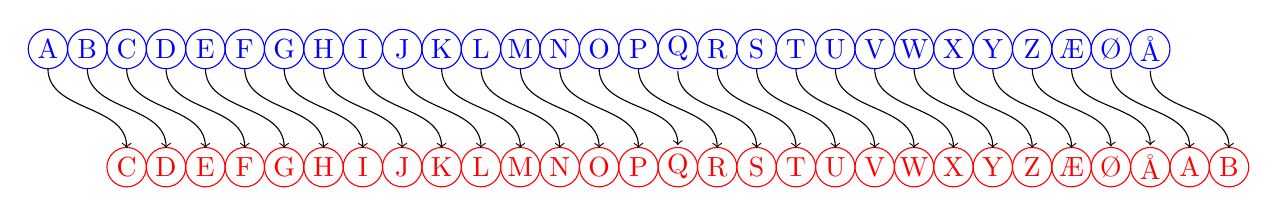
\begin{tikzpicture}
\foreach \i in {1,...,29}
{
     \draw[color=blue] (\i * 0.5 ,0) circle (0.25 cm);
}
\node[color = blue] at (0.5,0) (1) {A};
\node[color = blue] at (1,0) (2) {B};
\node[color = blue] at (1.5,0) (3) {C};
\node[color = blue] at (2,0) (4) {D};
\node[color = blue] at (2.5,0) (5) {E};
\node[color = blue] at (3,0) (6) {F};
\node[color = blue] at (3.5,0) (7) {G};
\node[color = blue] at (4,0) (8) {H};
\node[color = blue] at (4.5,0) (9) {I};
\node[color = blue] at (5,0) (10) {J};
\node[color = blue] at (5.5,0) (11) {K};
\node[color = blue] at (6,0) (12) {L};
\node[color = blue] at (6.5,0) (13) {M};
\node[color = blue] at (7,0) (14) {N};
\node[color = blue] at (7.5,0) (15) {O};
\node[color = blue] at (8,0) (16) {P};
\node[color = blue] at (8.5,0) (17) {Q};
\node[color = blue] at (9.0,0) (18) {R};
\node[color = blue] at (9.5,0) (19) {S};
\node[color = blue] at (10,0) (20) {T};
\node[color = blue] at (10.5,0) (21) {U};
\node[color = blue] at (11.0,0) (22) {V};
\node[color = blue] at (11.5,0) (23) {W};
\node[color = blue] at (12.0,0) (24) {X};
\node[color = blue] at (12.5,0) (25) {Y};
\node[color = blue] at (13,0) (26) {Z};
\node[color = blue] at (13.5,0) (27) {Æ};
\node[color = blue] at (14,0) (28) {Ø};
\node[color = blue] at (14.5,0) (29) {Å};

\foreach \i in {1,...,29}
{
     \draw[color=red] (\i * 0.5+1 ,-1.5) circle (0.25 cm);
}
\node[color = red] at (15,-1.5) (30) {A};
\node[color = red] at (15.5,-1.5) (31) {B};
\node[color = red] at (1.5,-1.5) (32) {C};
\node[color = red] at (2,-1.5) (33) {D};
\node[color = red] at (2.5,-1.5) (34) {E};
\node[color = red] at (3,-1.5) (35) {F};
\node[color = red] at (3.5,-1.5) (36) {G};
\node[color = red] at (4,-1.5) (37) {H};
\node[color = red] at (4.5,-1.5) (38) {I};
\node[color = red] at (5,-1.5) (39) {J};
\node[color = red] at (5.5,-1.5) (40) {K};
\node[color = red] at (6,-1.5) (41) {L};
\node[color = red] at (6.5,-1.5) (42) {M};
\node[color = red] at (7,-1.5) (43) {N};
\node[color = red] at (7.5,-1.5) (44) {O};
\node[color = red] at (8,-1.5) (45) {P};
\node[color = red] at (8.5,-1.5) (46) {Q};
\node[color = red] at (9.0,-1.5) (47) {R};
\node[color = red] at (9.5,-1.5) (48) {S};
\node[color = red] at (10,-1.5) (49) {T};
\node[color = red] at (10.5,-1.5) (50) {U};
\node[color = red] at (11.0,-1.5) (51) {V};
\node[color = red] at (11.5,-1.5) (52) {W};
\node[color = red] at (12.0,-1.5) (53) {X};
\node[color = red] at (12.5,-1.5) (54) {Y};
\node[color = red] at (13,-1.5) (55) {Z};
\node[color = red] at (13.5,-1.5) (56) {Æ};
\node[color = red] at (14,-1.5) (57) {Ø};
\node[color = red] at (14.5,-1.5) (58) {Å};

\draw[->] (1) to [out = -90,in = 90] (32);
\draw[->] (2) to [out = -90,in = 90] (33);
\draw[->] (3) to [out = -90,in = 90] (34);
\draw[->] (4) to [out = -90,in = 90] (35);
\draw[->] (5) to [out = -90,in = 90] (36);
\draw[->] (6) to [out = -90,in = 90] (37);
\draw[->] (7) to [out = -90,in = 90] (38);
\draw[->] (8) to [out = -90,in = 90] (39);

\draw[->] (9) to [out = -90,in = 90] (40);
\draw[->] (10) to [out = -90,in = 90] (41);
\draw[->] (11) to [out = -90,in = 90] (42);
\draw[->] (12) to [out = -90,in = 90] (43);

\draw[->] (13) to [out = -90,in = 90] (44);
\draw[->] (14) to [out = -90,in = 90] (45);
\draw[->] (15) to [out = -90,in = 90] (46);
\draw[->] (16) to [out = -90,in = 90] (47);

\draw[->] (17) to [out = -90,in = 90] (48);
\draw[->] (18) to [out = -90,in = 90] (49);
\draw[->] (19) to [out = -90,in = 90] (50);
\draw[->] (20) to [out = -90,in = 90] (51);

\draw[->] (21) to [out = -90,in = 90] (52);
\draw[->] (22) to [out = -90,in = 90] (53);
\draw[->] (23) to [out = -90,in = 90] (54);
\draw[->] (24) to [out = -90,in = 90] (55);

\draw[->] (25) to [out = -90,in = 90] (56);
\draw[->] (26) to [out = -90,in = 90] (57);

\draw[->] (27) to [out = -90,in = 90] (58);
\draw[->] (28) to [out = -90,in = 90] (30);

\draw[->] (29) to [out = -90,in = 90] (31);

\end{tikzpicture}
}
\caption{kryptering med Cæsar-chiffer hvor $k = 2$}
\label{fig:caesar}
\end{figure}
\begin{exa}
Vi modtager chifferteksten $c=$CPFGP G GNUMGT OCV, og vi ved, at den er krypteret med krypteringsfunktionen $e_2$. Derfor har vi, at 
\[
\textnormal{CPFGP G GNUMGT OCV} = e_2(m),
\]
hvor $m$ er klarteksten. For at finde $m$ bestemmer vi
\[
m = d_2(\textnormal{CPFGP G GNUMGT OCV}).
\]
Dette gøres ved at gå baglens i tabellen i Figur \ref{fig:caesar}, og vi får, at klarteksten er
\begin{align*}
m = \textnormal{ANDEN E ELSKER MAT}.
\end{align*}
\end{exa}
Med dette kryptosystem følger nogle ret store problemer. Hvis chifferteksten $c$ opsnappes af en tredjepart og tredjeparten ved, at beskeden er krypteret med et Cæsar-chiffer, så kan tredjeparten blot prøve alle 29 nøgler for at dekryptere. Dette kan højst tage 29 gange så lang tid som at dekryptere en besked, hvis man ikke kender nøglen, som hvis man kender den, hvilket er alt for kort tid. 

Alternativt kunne man parre bogstaverne på andre måder. Dette ville øge sikkerheden mod et angreb, der består i at afprøve alle nøgler, da man kan parre bogstaverne på 
\[
29! = 8841761993739701954543616000000
\]
måder. Men så kan man udnytte strukturen i en gennemsnitlig tekst. På dansk er det hyppigst brugte bogstav E, der optræder som omtrent $15\%$ af alle bogstaver. Derfor vil det hyppigste bogstav i en chiffertekst formentlig tilsvare E i klarteksten. Denne analyse kan så gennemgåes med det næsthyppigste bogstav, tredjehyppigste osv. indtil chifferteksten kan dechifreres til klarteksten. 

Et kryptosystem som Cæsar-chifferet kaldes for et symmetrisk kryptosystem, da begge parter skal blive enige om en krypteringsnøgle $k$. 

Vi bemærker, at man kan beskrive Cæsar-chifferet ved moduloregning. Gives alle bogstaver et tal, fx A = 1, B = 2, osv., så tilsvarer en forskydning på $k$ bogstaver at lægge $k$ til hvert symbol$\fmod{29}$. Krypteringen af HEJ (8 5 10) med nøglen $k = 20$ vil tilsvare
\begin{align*}
	&8 + 20 \fmod{29} = 28\\
	&5 + 20 \fmod{29} = 25\\
	&10 + 20 \fmod{29} = 1\\
\end{align*}
Den krypterede besked vil derfor være (28 25 1), altså ÆYA.

